As mentioned in Chapter.~\ref{chap:intro}, array processing serves in many different application, each with its unique requirements, setup and constraints - hence performance criteria are application dependent.
In this work, we focus on localization related applications and suggest a new architecture.
Hence, to analyse the presented scheme, we use classic localization-related performance measurements as the comparison is to known localization related array processing schemes.
\par
To this end, we follow the classic \cite{van2004optimum} performance analysis, elaborated in the following.
Those criteria are then used to quantify the presented architecture's performance in Chapter.\ref{chap:firstchap}.
\subsection{Beampattern}
Considering DOA estimators, the main tool for assessing an array's localization performance is expressing it's response to impinging signals with respect to the signal's DOA.
\begin{figure}
  \centering
  \begin{subfigure}[b]{0.49\linewidth}
    % 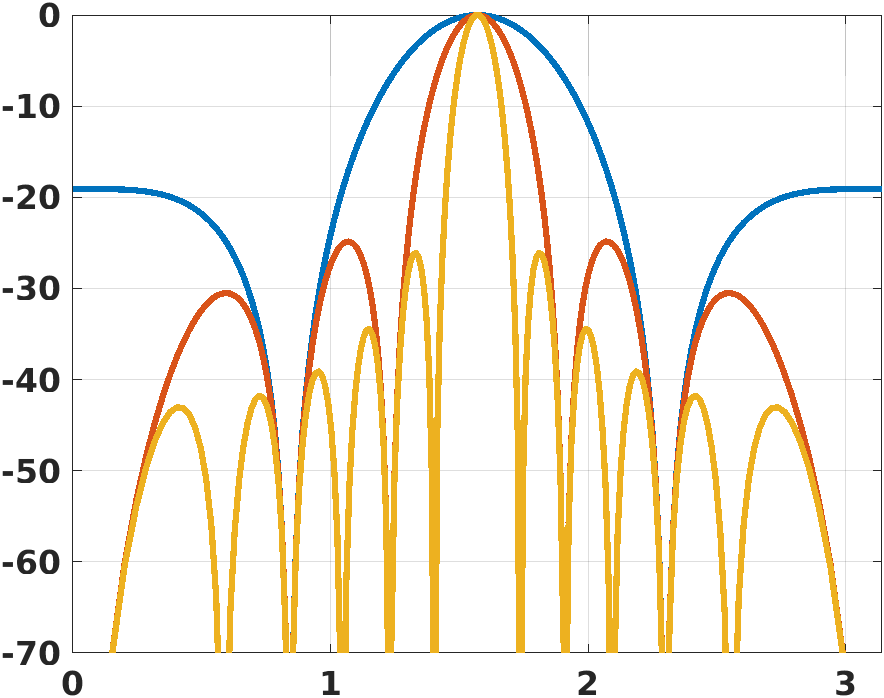
\includegraphics[width=\linewidth]{./Media/fig_commonBp_1.png}
    \begin{overpic}[width=\linewidth, 
        %grid, 
        tics=10,trim=0 0 0 0]{./Media/fig_commonBp_1.png}
            \put (19, 58){\tiny{$N\!=\!3$}}
            \put (19, 47){\tiny{$N\!=\!6$}}
            \put (19, 34){\tiny{$N\!=\!12$}}
    \end{overpic}
    \caption{}
    \label{fig_common_bps1}
  \end{subfigure}
  %
  \begin{subfigure}[b]{0.4\linewidth}
    \begin{overpic}[width=\linewidth, 
        %grid, 
        tics=10,trim=0 0 0 0]{./Media/fig_commonBp_2.png}
            \put (81, 63.5){\tiny{$N\!=\!3$}}
            \put (76, 57){\tiny{$N\!=\!6$}}
            \put (76, 53){\tiny{$N\!=\!12$}}
    \end{overpic}
    \caption{}
    \label{fig_common_bps2}
  \end{subfigure}
  \caption{Two common ways of visualizing the array's response in the 2D planar case.
  In both plots, a comparison between the conventional beamformer's responses of 3,6 and 12 elements arrays is emulated. 
  In Fig.~\ref{fig_common_bps1}, the response is presented on the interval of 0 to $\pi$ with units of dB.
  In Fig.~\ref{fig_common_bps2}, a polar plot is presented with same units for the response gain but the DOA is in degrees.}
  \label{fig_common_bps}
\end{figure}
Although may be dependant in various parameters, for the sake of simplicity, we consider a planar (i.e. azimuth without elevation) DOA-only dependant array response (i.e. the \emph{beampattern})
\begin{equation}
B\rBrace{\theta} = 20\log_{10}\abs{Z\rBrace{\theta}}.
\end{equation}
The beampttern is commonly presented in a graphical manner as exemplified in Fig.~\ref{fig_common_bps}.
It's characteristics, such as lobes width, attenuation and positioning are then analysed and compared between different schemes.
The analysis can theoretical, when the beampattern's mathematical expression is known or graphical analysis for empirical scenarios.
In this work, as we deal with 2D planar localization problems, we find the presentation of Fig.~\ref{fig_common_bps1} most suitable.
The horizontal axis, being the DOAs of the impinging signal, may be presented in various ways where units may be degrees radians etc.
Also, as the DOA is periodical one should also choose the centering, for example when the beampattern is steered towards different angles and the author wants to center the mainlobe.
In this work, we follow choose to use \cite{van2004optimum}'s $\psi$-space, i.e.
\begin{equation}
    \psi\rBrace{\theta_{d}}=\frac{2\pi}{\lambda}\cos{\theta_{d}}\cdot{}d,
\end{equation}
where $\lambda$ is the impinging signal's wavelength.
The reader may notice that $\psi$ is exactly the electric phase $\theta$ defined in \eqref{eq:thetaULA}. 
Also, we choose to plot beampatterns using $\Delta\psi = \psi\rBrace{\theta_{d}} - \psi\rBrace{\theta_{s}}$, where $\theta_{s}$ is the steering angle of the array, for it centers the mainlobe, enabling convenient comparison.
\subsection{The normalized beampattern}
As the absolute output gain is system dependent, comparing two different is not possible where their maximal gain of the mainlobe are different.
Therefore, a common practice \cite{van2004optimum} when analysing the array's spatial performance, is to normalize the beampattern such that the mainlobe's output gain at it's peak is 1 (0dB), thus enabling convenient comparable measures extraction.
This quantity will be referred as $\mathcal{H}$.
\subsection{Half power beamwidth}
Considering localization problems, possibly the main interest is spatial resolution, related to localization accuracy and distinction of spatially close objects, where ``close`` can be interpreted as small physical distance between objects of interest or objects that may be physically distant from each other but from the array's perspective are in relatively similar.
\par
Relating to the beampttern, the spatial resolution is obviously linked to the main lobe's width, i.e. higher resolution is acheived as the main lobe thins. 
Hence to unify the analysis, the Half Power BeamWidth (HPBW) is defined to be the 3-dB beamwidth, i.e. the point where $\abs{B\rBrace{\psi}}^{2} = 0.5$ or $\abs{B\rBrace{\psi}} = 1/\sqrt{2}$.
For standard ULA, assuming large $N$ values, it is known \cite{van2004optimum} that
\begin{equation}
    \label{eq_known_HBPW}
    \dThetaHPBW/2= 1.4/N.
\end{equation}
\par
Obviously, we aim to show that the presented architecture increases the resolution, comparing to other arrays by proving that the beamwidth shrinks.
%
%
%
\subsection{Sidelobes attenuation}
As the beampattern consists of multiple harmonics (as the number of elements $N$), sidelobes occur when the some harmonics are summed, showing as peaks other than the mainlobe.
As this is an unwanted result, the height and their rate of decrease are measured aiming to prefer arrays where their height is reduced and the decrease rate is increased.
%
%
%
\subsection{Directivity}
The array directivity $\mathcal{D}$ \cite{van2004optimum}, defined as
\begin{equation}\label{eq_D}
    \mathcal{D}\rBrace{N,r} = \frac{\Hr_{\Delta\theta=0,\Delta\phi=0,r}}{\frac{1}{2\pi}\int_{0}^{2\pi}\Hr_{\Delta\theta,\Delta\phi=0,r}\ d\Delta\theta} = \frac{2\pi}{\int_{0}^{2\pi}\Hr_{\Delta\theta,\Delta\phi=0,r}\ d\Delta\theta},
\end{equation}
measures the ratio between the maximal array gain at its mainlobe, to the average gain over all directions. 
For uniformly weighted ULAs with no feedback, it is known \cite{van2004optimum} that $\mathcal{D}\rBrace{N,0} = N$.
